%% This file was auto-generated by IPython.
%% Conversion from the original notebook file:
%% svdcluster2.ipynb
%%
\documentclass[11pt,english,fleqn]{article}

%% This is the automatic preamble used by IPython.  Note that it does *not*
%% include a documentclass declaration, that is added at runtime to the overall
%% document.

\usepackage{amsmath}
\usepackage{amssymb}
\usepackage{graphicx}
\usepackage{ucs}
\usepackage[utf8x]{inputenc}

% needed for markdown enumerations to work
\usepackage{enumerate}

% Slightly bigger margins than the latex defaults
\usepackage{geometry}
\geometry{verbose,tmargin=3cm,bmargin=3cm,lmargin=2.5cm,rmargin=2.5cm}

% Define a few colors for use in code, links and cell shading
\usepackage{color}
\definecolor{orange}{cmyk}{0,0.4,0.8,0.2}
\definecolor{darkorange}{rgb}{.71,0.21,0.01}
\definecolor{darkgreen}{rgb}{.12,.54,.11}
\definecolor{myteal}{rgb}{.26, .44, .56}
\definecolor{gray}{gray}{0.45}
\definecolor{lightgray}{gray}{.95}
\definecolor{mediumgray}{gray}{.8}
\definecolor{inputbackground}{rgb}{.95, .95, .85}
\definecolor{outputbackground}{rgb}{.95, .95, .95}
\definecolor{traceback}{rgb}{1, .95, .95}

% Framed environments for code cells (inputs, outputs, errors, ...).  The
% various uses of \unskip (or not) at the end were fine-tuned by hand, so don't
% randomly change them unless you're sure of the effect it will have.
\usepackage{framed}

% remove extraneous vertical space in boxes
\setlength\fboxsep{0pt}

% codecell is the whole input+output set of blocks that a Code cell can
% generate.

% TODO: unfortunately, it seems that using a framed codecell environment breaks
% the ability of the frames inside of it to be broken across pages.  This
% causes at least the problem of having lots of empty space at the bottom of
% pages as new frames are moved to the next page, and if a single frame is too
% long to fit on a page, will completely stop latex from compiling the
% document.  So unless we figure out a solution to this, we'll have to instead
% leave the codecell env. as empty.  I'm keeping the original codecell
% definition here (a thin vertical bar) for reference, in case we find a
% solution to the page break issue.

%% \newenvironment{codecell}{%
%%     \def\FrameCommand{\color{mediumgray} \vrule width 1pt \hspace{5pt}}%
%%    \MakeFramed{\vspace{-0.5em}}}
%%  {\unskip\endMakeFramed}

% For now, make this a no-op...
\newenvironment{codecell}{}

 \newenvironment{codeinput}{%
   \def\FrameCommand{\colorbox{inputbackground}}%
   \MakeFramed{\advance\hsize-\width \FrameRestore}}
 {\unskip\endMakeFramed}

\newenvironment{codeoutput}{%
   \def\FrameCommand{\colorbox{outputbackground}}%
   \vspace{-1.4em}
   \MakeFramed{\advance\hsize-\width \FrameRestore}}
 {\unskip\medskip\endMakeFramed}

\newenvironment{traceback}{%
   \def\FrameCommand{\colorbox{traceback}}%
   \MakeFramed{\advance\hsize-\width \FrameRestore}}
 {\endMakeFramed}

% Use and configure listings package for nicely formatted code
\usepackage{listingsutf8}
\lstset{
  language=python,
  inputencoding=utf8x,
  extendedchars=\true,
  aboveskip=\smallskipamount,
  belowskip=\smallskipamount,
  xleftmargin=2mm,
  breaklines=true,
  basicstyle=\small \ttfamily,
  showstringspaces=false,
  keywordstyle=\color{blue}\bfseries,
  commentstyle=\color{myteal},
  stringstyle=\color{darkgreen},
  identifierstyle=\color{darkorange},
  columns=fullflexible,  % tighter character kerning, like verb
}

% The hyperref package gives us a pdf with properly built
% internal navigation ('pdf bookmarks' for the table of contents,
% internal cross-reference links, web links for URLs, etc.)
\usepackage{hyperref}
\hypersetup{
  breaklinks=true,  % so long urls are correctly broken across lines
  colorlinks=true,
  urlcolor=blue,
  linkcolor=darkorange,
  citecolor=darkgreen,
  }

% hardcode size of all verbatim environments to be a bit smaller
\makeatletter 
\g@addto@macro\@verbatim\small\topsep=0.5em\partopsep=0pt
\makeatother 

% Prevent overflowing lines due to urls and other hard-to-break entities.
\sloppy

\setlength{\mathindent}{0pt}
\setlength{\parindent}{0pt}
\setlength{\parskip}{8pt}
\begin{document}

SVD ile Kumeleme

Tekil Deger Ayristirma (Singular Value Decomposition -SVD-) ile bir veri
madenciligi ornegi gorecegiz. Ornek olarak {[}1{]} adresinde tarif
edilen / paylasilan zaman serisini kullandik. Serinin tumunu
kullanilmadi, ilk 10 noktasini aldik, ve grafige bakinca iki tane ana
seri turu oldugunu goruyoruz.

\begin{codecell}
\begin{codeinput}
\begin{lstlisting}
import numpy as np
data = np.genfromtxt("synthetic_control.data", dtype=float)

print data.shape

for t in data[:,0:10]:
    plot(t); hold(True)

\end{lstlisting}
\end{codeinput}
\begin{codeoutput}
\begin{verbatim}
(600, 60)
\end{verbatim}
\begin{center}
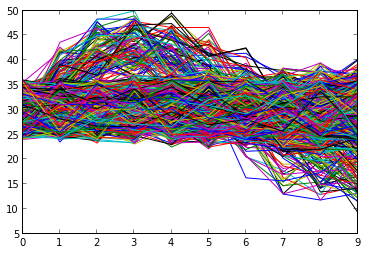
\includegraphics[width=0.7\textwidth]{svdcluster2_files/svdcluster2_fig_00.png}
\par
\end{center}
\end{codeoutput}
\end{codecell}
Peki bu serileri nasil otomatik olarak kumeleyerek bulurduk /
birbirinden ayirtederdik? \emph{Lineer Cebir Ders 29}'da SVD'nin
matematigini isledik. SVD bir matris $A$ uzerinde ayristirma yapar, ve
$A$ herhangi boyutta, turde bir matris olabilir.

\begin{codecell}
\begin{codeinput}
\begin{lstlisting}
im=imread("svd1.png"); imshow(im)
\end{lstlisting}
\end{codeinput}
\begin{codeoutput}
\begin{verbatim}
<matplotlib.image.AxesImage at 0xabc91ac>
\end{verbatim}
\begin{center}
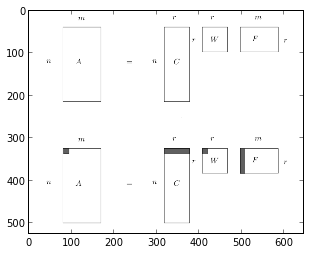
\includegraphics[width=0.7\textwidth]{svdcluster2_files/svdcluster2_fig_01.png}
\par
\end{center}
\end{codeoutput}
\end{codecell}
Ayristirma $m \times n$ boyutlu matrisi $A=CWF$ olarak ayristirir,
burada $C$, ana matris ile ayni miktarda satira sahiptir, $F$ ayni
miktarda kolona sahiptir. Ayristirma sonrasi $A$'nin kertesi (rank) $r$
ortaya cikar, eger tum $A$ kolonlari birbirinden bagimsiz ise, o zaman
$r=m$ olacaktir, ama kolonlarin bazilari mesela ayni olcumu degisik
katlarda tekrarliyor ise, o zaman matriste tekillik vardir, ve bu
durumda $r < m$ olur, ve ortadaki $W$ matrisi $r \times r$ oldugu icin
beklenenden daha ufak boyutlarda olabilir.

Ayrica SVD, $W$ caprazindaki ozdegerleri buyukluk sirasina gore dizer,
ve her ozdegere tekabul eden ozvektorler de ona gore siraya dizilmis
olacaktir, ve SVD tamamlaninca mesela ``en buyuk 10'' ozdegere ait olan
$CWF$ degerlerini alip, digerlerini atmayi da secebiliriz, yani kerte
uzerinden yapilan ``eleme'' ustune bir eleme de kendimiz yapabiliriz. Bu
elemeyi yapabilmemizin mantigi soyle; kucuk ozdegerlerin carptigi
ozvektorlerin nihai toplama daha az etki ettigi soylenebilir, ve bu
``gurultuyu'' elemek sonucu degistirmeyecektir. Ayrica bu elemeyi
yaparak bir tur boyut azaltma (dimensionality reduction) islemini de
ayni zamanda basarmis oluruz.

Ayristirmanin Anlamlari

Bir ayristirmayi degisik sekillerde gormek mumkundur. Bunlardan onemli
birisi cizge bakis acisidir (graph interpretation). Cizge bilindigi gibi
dugumler ve onlar arasindaki ayritlardan (edges) olusur. Bir cizge
matris formunda temsil edilebilir, satir / kolon kesisimi iki dugum
arasindaki ayritin agirligini, ya da varligini (1 ve 0 uzerinden) temsil
edecektir. Bu durumda SVD sonucunda elde edilen $CWF$, bize iki dugum
arasi gecisli (bipartite) cizgeyi, uc dugum arasi gecisli (tripartite)
cizgeye cevrilmis halde geri verir. Ve bu yeni cizgede en fazla $r$ tane
gecis noktalari (waystations) olusmustur, ustte bahsettigimiz eleme ile
gecisler daha da azaltilabilir.

Simdi, bu gecis noktalarina olan $C$`nin ``baglanma sekli'', ``baglanma
kuvveti'', ek kumeleme basamagi tarafindan kullanilabilir. Bu
``azaltilmis'' gecisin uzerindeki her islem / ona yapilan her referans
kumeleme icin bir ipucudur. Bunu gormek icin ornek zaman serilerinin SVD
sonrasi elde edilen $C$ (ornekte u) matrisinin ilk iki kolonunu bile
grafiklemek yeterlidir.

\begin{codecell}
\begin{codeinput}
\begin{lstlisting}
import scipy.linalg as lin
data = np.genfromtxt("synthetic_control.data", dtype=float)

# before norm, and take only 10 data points
data = data[:,0:10]

print data.shape

# show the mean, and std of the first time series
print data[0,:]
print np.mean(data[0,:], axis=0)
print np.std(data[0,:], axis=0)

# normalize
data -= np.mean(data, axis=0)
data /= np.std(data, axis=0)

# after norm
print data[0,:]

u,s,v = lin.svd(data, full_matrices=False)
print 'svd'
print u.shape
print s
print v.shape

plot(u[:,0], u[:,1], '.')

\end{lstlisting}
\end{codeinput}
\begin{codeoutput}
\begin{verbatim}
(600, 10)
[ 28.7812  34.4632  31.3381  31.2834  28.9207  33.7596  25.3969  27.7849
  35.2479  27.1159]
30.40918
3.16894521278
[-0.35501371  0.85457443 -0.10641642 -0.16202975 -0.51986031  0.56762802
 -1.19371757 -0.29304061  1.27639519 -0.2095089 ]
svd
(600, 10)
[ 48.29293361  30.97232928  24.52860861  20.63081553  20.0940039
  17.52035809  16.48932523  16.03796372  15.41270426  14.27678793]
(10, 10)
\end{verbatim}
\begin{verbatim}
[<matplotlib.lines.Line2D at 0xc131d4c>]
\end{verbatim}
\begin{center}
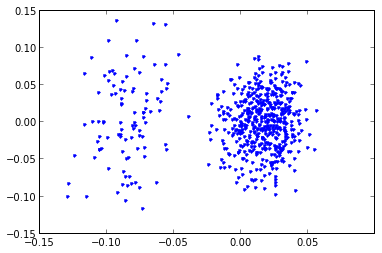
\includegraphics[width=0.7\textwidth]{svdcluster2_files/svdcluster2_fig_02.png}
\par
\end{center}
\end{codeoutput}
\end{codecell}
Goruldugu gibi net bir sekilde iki tane kume ortaya cikti. Bu kumeler
yazinin basindaki iki ayri zaman serisi obeklerine tekabul ediyorlar.

O zaman serilerini ayirtetmek icin ne yapariz? Ustteki veriler uzerinde
kmeans isletebilirdik, ya da kabaca bakiyoruz, dikey olarak -0.025
seviyesinde bir cizgi ayirac olarak gorulebilir. Numpy filtreleme
teknigi

 u{[}:,0{]} \textless{} -0.025

bize ana veri uzerinde uygulanabilecek True ve False degerleri verir,
bunlari alarak ana veriye filtrele olarak uygulariz,

 data{[}u{[}:,0{]} \textless{} -0.025{]}

ve mesela birinci kumeye ait zaman serilerini bulabiliriz.

Kontrol etmek icin ilk 3 kolonun degerlerini uc boyutta grafikleyelim.

\begin{codecell}
\begin{codeinput}
\begin{lstlisting}
from mpl_toolkits.mplot3d import Axes3D
import scipy.linalg as lin

data = np.genfromtxt("synthetic_control.data", dtype=float)

data = data[:,0:10]

print data.shape

data -= np.mean(data, axis=0)
data /= np.std(data, axis=0)

u,s,v = lin.svd(data)
print 'svd'
print u.shape
print s
print v.shape

fig = plt.figure()
ax = Axes3D(fig)
ax.plot(u[:,0], u[:,1], u[:,2],',', zs=0, zdir='z', label='zs=0, zdir=z')

\end{lstlisting}
\end{codeinput}
\begin{codeoutput}
\begin{verbatim}
(600, 10)
svd
(600, 600)
[ 48.29293361  30.97232928  24.52860861  20.63081553  20.0940039
  17.52035809  16.48932523  16.03796372  15.41270426  14.27678793]
(10, 10)
\end{verbatim}
\begin{verbatim}
[<mpl_toolkits.mplot3d.art3d.Line3D at 0xbe5ec6c>]
\end{verbatim}
\begin{center}
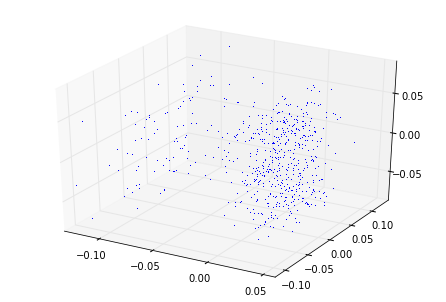
\includegraphics[width=0.7\textwidth]{svdcluster2_files/svdcluster2_fig_03.png}
\par
\end{center}
\end{codeoutput}
\end{codecell}
Yine iki tane kume oldugunu goruyoruz.

Simdi biraz daha degisik bir probleme bakalim, bu sefer bir grup
kelimeyi birbirlerine benzerlikleri (ya da uzakligi) uzerinden
kumelemeye ugrasacagiz.

Benzerlik, Levenhstein mesafesi adli olcut {[}2{]} uzerinden olacak.
Matrisimiz her kelimenin her diger kelime ile arasindaki uzakligi veren
bir matris olmali, eger 100 kelime var ise, bu matris 100 x 100
boyutlarinda olacak. SVD sonrasi elde edilen u uzerinde kmeans
isletecegiz, ve kumeleri bulacagiz. Ayrica her kume icin bir
``temsilci'' secebilmek icin kmeans'in bize verdigi kume ortasi
kordinatinin en yakin oldugu kelimeyi cekip cikartacagiz, ve onu
temsilci olarak alacagiz.

\begin{codecell}
\begin{codeinput}
\begin{lstlisting}
import scipy.linalg as lin
import Levenshtein as leven
from sklearn.cluster import KMeans
import itertools

words = np.array(
    ['the', 'be', 'to', 'of', 'and', 'a', 'in', 'that', 'have',
     'I', 'it', 'for', 'not', 'on', 'with', 'he', 'as', 'you',
     'do', 'at', 'this', 'but', 'his', 'by', 'from', 'they', 'we',
     'say', 'her', 'she', 'or', 'an', 'will', 'my', 'one', 'all',
     'would', 'there', 'their', 'what', 'so', 'up', 'out', 'if',
     'about', 'who', 'get', 'which', 'go', 'me', 'when', 'make',
     'can', 'like', 'time', 'no', 'just', 'him', 'know', 'take',
     'people', 'into', 'year', 'your', 'good', 'some', 'could',
     'them', 'see', 'other', 'than', 'then', 'now', 'look',
     'only', 'come', 'its', 'over', 'think', 'also', 'back',
     'after', 'use', 'two', 'how', 'our', 'work', 'first', 'well',
     'way', 'even', 'new', 'want', 'because', 'any', 'these',
     'give', 'day', 'most', 'us'])

print "calculating distances..."

(dim,) = words.shape

f = lambda (x,y): leven.distance(x,y)

res=np.fromiter(itertools.imap(f, itertools.product(words, words)),
                dtype=np.uint8)
A = np.reshape(res,(dim,dim))

print "svd..."

u,s,v = lin.svd(A, full_matrices=False)

print u.shape
print s.shape
print s
print v.shape

data = u[:,0:8]
k=KMeans(init='k-means++', n_clusters=25, n_init=10)
k.fit(data)
centroids = k.cluster_centers_
labels = k.labels_
print labels

def dist(x,y):   
    return np.sqrt(np.sum((x-y)**2, axis=1))
    
print "clusters, centroid points.."
for i,c in enumerate(centroids):
    idx = np.argmin(dist(c,data[labels==i]))
    print words[labels==i][idx]
    print words[labels==i]
    
plt.plot(centroids[:,0],centroids[:,1],'x')
plt.hold(True)
plt.plot(u[:,0], u[:,1], '.')
plt.show()

from mpl_toolkits.mplot3d import Axes3D
fig = plt.figure()
ax = Axes3D(fig)
ax.plot(u[:,0], u[:,1], u[:,2],'.', zs=0,
        zdir='z', label='zs=0, zdir=z')
\end{lstlisting}
\end{codeinput}
\begin{codeoutput}
\begin{verbatim}
calculating distances...
svd...
(100, 100)
(100,)
[  3.57988202e+02   4.64912561e+01   3.21352688e+01   2.38031643e+01
   2.14888993e+01   1.75355875e+01   1.72577475e+01   1.50823345e+01
   1.36053187e+01   1.27864289e+01   1.20850058e+01   1.09366461e+01
   1.02722223e+01   9.15906107e+00   8.93781797e+00   8.08808906e+00
   7.55885762e+00   7.38765898e+00   7.03189413e+00   6.37905207e+00
   6.08100883e+00   5.93978699e+00   5.80476820e+00   5.48573127e+00
   4.93815941e+00   4.58515335e+00   4.40072056e+00   4.10393093e+00
   3.82184278e+00   3.62002998e+00   3.52076475e+00   3.21765568e+00
   3.19448751e+00   2.97591545e+00   2.90604264e+00   2.82566873e+00
   2.75236845e+00   2.51068720e+00   2.46909289e+00   2.39525952e+00
   2.31057708e+00   2.17681774e+00   2.11768873e+00   2.02116412e+00
   1.99158340e+00   1.84283752e+00   1.80985462e+00   1.73585790e+00
   1.59395705e+00   1.57675090e+00   1.49638568e+00   1.49354064e+00
   1.40623601e+00   1.40412600e+00   1.24442892e+00   1.23842955e+00
   1.22119742e+00   1.20466658e+00   1.19604521e+00   1.08815700e+00
   9.78864620e-01   9.71322173e-01   8.83519026e-01   8.53898791e-01
   8.53690716e-01   7.32954748e-01   7.14196035e-01   6.92366775e-01
   6.83931613e-01   5.88533124e-01   5.45586737e-01   5.01747612e-01
   4.90740691e-01   4.29689160e-01   4.09996636e-01   4.03042824e-01
   3.80587104e-01   3.48811148e-01   3.28580353e-01   3.25050141e-01
   3.09318382e-01   2.39526940e-01   2.29926274e-01   1.96030630e-01
   1.86987383e-01   1.46740385e-01   1.44728633e-01   1.30118418e-01
   1.28613583e-01   8.03675410e-02   6.31950264e-02   5.25562558e-02
   3.08220025e-02   2.85652995e-02   2.84199001e-02   4.43547511e-03
   1.60953158e-04   3.44433012e-14   3.44433012e-14   3.44433012e-14]
(100, 100)
[ 4  0 23  1  3 19  9 14 12 20  9 15 15  1  5  0 19 15 23 19 14 21  9 20  8
  4  0  3 22  0  1  3  5 20  1 10  6 22 22 10 23 20 21  9  2  7 20  5 23  0
  4 12  3 11 11 23  2  7  8 12 13  7 18  6  8 13  6  4  0 22 14  4 15  8 17
 13  9 18 14  2 10 18  0 23 15 21 17  2 17 10 18  1 10 16  3 24 11  3  2 20]
\end{verbatim}
\begin{verbatim}
clusters, centroid points..
be
['be' 'he' 'we' 'she' 'me' 'see' 'use']
of
['of' 'on' 'or' 'one' 'new']
most
['about' 'just' 'also' 'first' 'most']
day
['and' 'say' 'an' 'can' 'any' 'day']
they
['the' 'they' 'when' 'them' 'then']
with
['with' 'will' 'which']
could
['would' 'your' 'could']
into
['who' 'him' 'into']
look
['from' 'know' 'good' 'look']
if
['in' 'it' 'his' 'if' 'its']
want
['all' 'what' 'back' 'way' 'want']
like
['like' 'time' 'give']
have
['have' 'make' 'take']
come
['people' 'some' 'come']
that
['that' 'this' 'than' 'think']
not
['for' 'not' 'you' 'now' 'how']
because
['because']
only
['only' 'work' 'well']
even
['year' 'over' 'after' 'even']
at
['a' 'as' 'at']
I
['I' 'by' 'my' 'up' 'get' 'us']
out
['but' 'out' 'our']
other
['her' 'there' 'their' 'other']
do
['to' 'do' 'so' 'go' 'no' 'two']
these
['these']
\end{verbatim}
\begin{center}
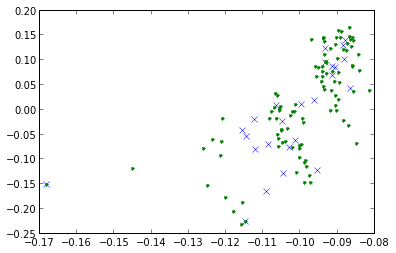
\includegraphics[width=0.7\textwidth]{svdcluster2_files/svdcluster2_fig_04.png}
\par
\end{center}
\begin{verbatim}
[<mpl_toolkits.mplot3d.art3d.Line3D at 0xbe01bac>]
\end{verbatim}
\begin{center}
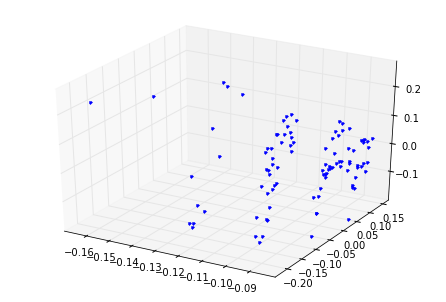
\includegraphics[width=0.7\textwidth]{svdcluster2_files/svdcluster2_fig_05.png}
\par
\end{center}
\end{codeoutput}
\end{codecell}
Bu teknigin uygulanabilecegi daha pek cok alan var. Mesela her dokumanin
icindeki belli kelimelerin sayilari kolonlarda (her kolon ozel bir
kelimeye tekabul edecek sekilde), ve dokumanlarin kendisi satirlarda
olacak sekilde bir matrisimiz olsaydi, SVD bu matris uzerinde de bir
kumeleme icin kullanilabilirdi. Bu ornekte ``kac tane kelime oldugu''
gibi bir olcut vardir (daha once kelimelerin birbirine uzakligini
kullandik), ama teknik yine de ise yarar.

{[}1{]}
http://kdd.ics.uci.edu/databases/synthetic\_control/synthetic\_control.data.html

{[}2{]}
http://sayilarvekuramlar.blogspot.de/2012/07/kelime-benzerligi-levenshtein-mesafesi.html

{[}3{]} Skillicorn, D., Understanding Complex Datasets Data Mining with
Matrix Decompositions

\end{document}
